%%%%%%%%%%%%%%%%%%%%%%%%%%%%%%%%%%%%%%%%%
% Beamer Presentation
% LaTeX Template
% Version 2.0 (10/06/16)
%
% Attention:
% 0. The self-defined font is used, because 'Calibri' is 
% not supported in the latex font packages. 'LuaLatex'
% should be used.
% 1. This template has been generated according to 
% the Power Point template of LUMC in 2016. 
% 2. This is generated purely with images as the 
% background.
% 3. The bullet point color was used purely for personal 
% preference. 
% 4. Any more adding to the template are welcome. 
% 5.In order to use the navigation bar, the title 
% for each section should not be to long. 
% 6.Adding animation is possible. I prefer to add another
% pdf file with:
% \animategraphics[parameters]{1}{fname}{startnum}{endnum}
% 7. This is my first template, the files might be not  
% well organized, sorry for that. 
% 
% Author:
% Shengnan Liu
% sliu729@gmail.com
% Division Medical imaging processing, 
% Leiden University Medical Center
% 
%%%%%%%%%%%%%%%%%%%%%%%%%%%%%%%%%%%%%%%%%
% Modification Log:
% Generated by Shengnan Liu on 21-01-2016
% Cleaned up for further usage on 10-06-2016
%%%%%%%%%%%%%%%%%%%%%%%%%%%%%%%%%%%%%%%%%
\documentclass[aspectratio=169]{beamer}
\title{Holistic Sleep Medicine 全人睡眠醫學}
\date[today]{\today}
\author[Name]{祁力行}
\institute[Oral and Maxillofacial Surgery]{Wan Fang Hospital, Taipei Medical University}
\usetheme{lumc}% theme

\usepackage{ifthen} % for If with condition: \ifthenelse{condition}{A}{B}

\usepackage{adjustbox} % for minipage to the right

\usepackage{tabularx} % for resizebox?

%\usepackage{CJKutf8} % by pdfLaTeX, not LuaLaTeX
% *** https://www.math.sinica.edu.tw/www/tex/default14.jsp
\usepackage{xeCJK} % for Chinese, compiling by XeLaTex

\usepackage{fontspec} %設定字體
% Fandol font (the default)  not shown "內"
\setCJKmainfont{AR PL UMing TW MBE} % AR PL UMing TW MBE or "UKai" https://www.overleaf.com/learn/latex/Questions/Which_OTF_or_TTF_fonts_are_supported_via_fontspec%3F#Chinese
%BiauKai} %標楷體 from macOS %設定中文為系統上的字型,而英文不去更動,使用原TeX字型

\XeTeXlinebreaklocale "zh"
\XeTeXlinebreakskip = 0pt plus 1pt %這兩行一定要加,中文才能自動換行

\usepackage{outlines}
\usepackage{booktabs}
% for tikz and gantt

\usepackage{pgfgantt} % for Gantt chart/flow chart
\definecolor{barblue}{RGB}{153,204,254}
\definecolor{groupblue}{RGB}{51,102,254}
\definecolor{linkred}{RGB}{165,0,33}

\usepackage{newfloat} % for caption of smartdiagram
\DeclareFloatingEnvironment[fileext=diag,placement={!ht},name=Figure ]{diag} % diag

\usepackage{smartdiagram} %flowchart
\usesmartdiagramlibrary{additions} 
\usepackage{tikz}   % for DAG plot by  tikzpicture
\usetikzlibrary{shadings,shadows,shapes.arrows,decorations.text,arrows.meta,bending}
%\usetikzlibrary{arrows}
%% This is not an official TikZ library. Use at your own risk!
% https://tex.stackexchange.com/questions/5461/is-it-possible-to-change-the-size-of-an-arrowhead-in-tikz-pgf

\makeatletter
% alternative latex arrow
\pgfarrowsdeclare{latexnew}{latexnew}
{
  \ifdim\pgfgetarrowoptions{latexnew}=-1pt%
    \pgfutil@tempdima=0.28pt%
    \pgfutil@tempdimb=\pgflinewidth%
    \ifdim\pgfinnerlinewidth>0pt%
      \pgfmathsetlength\pgfutil@tempdimb{.6\pgflinewidth-.4*\pgfinnerlinewidth}%
    \fi%
    \advance\pgfutil@tempdima by.3\pgfutil@tempdimb%
  \else%
    \pgfutil@tempdima=\pgfgetarrowoptions{latexnew}%
    \divide\pgfutil@tempdima by 10%
  \fi%
  \pgfarrowsleftextend{+-1\pgfutil@tempdima}%
  \pgfarrowsrightextend{+9\pgfutil@tempdima}%
}
{
  \ifdim\pgfgetarrowoptions{latexnew}=-1pt%
    \pgfutil@tempdima=0.28pt%
    \pgfutil@tempdimb=\pgflinewidth%
    \ifdim\pgfinnerlinewidth>0pt%
      \pgfmathsetlength\pgfutil@tempdimb{.6\pgflinewidth-.4*\pgfinnerlinewidth}%
    \fi%
    \advance\pgfutil@tempdima by.3\pgfutil@tempdimb%
  \else%
    \pgfutil@tempdima=\pgfgetarrowoptions{latexnew}%
    \divide\pgfutil@tempdima by 10%
    \pgfsetlinewidth{0bp}%
  \fi%
  \pgfpathmoveto{\pgfqpoint{9\pgfutil@tempdima}{0pt}}
  \pgfpathcurveto
  {\pgfqpoint{6.3333\pgfutil@tempdima}{.5\pgfutil@tempdima}}
  {\pgfqpoint{2\pgfutil@tempdima}{2\pgfutil@tempdima}}
  {\pgfqpoint{-1\pgfutil@tempdima}{3.75\pgfutil@tempdima}}
  \pgfpathlineto{\pgfqpoint{-1\pgfutil@tempdima}{-3.75\pgfutil@tempdima}}
  \pgfpathcurveto
  {\pgfqpoint{2\pgfutil@tempdima}{-2\pgfutil@tempdima}}
  {\pgfqpoint{6.3333\pgfutil@tempdima}{-.5\pgfutil@tempdima}}
  {\pgfqpoint{9\pgfutil@tempdima}{0pt}}
  \pgfusepathqfill
}

% alternative latex reversed arrow
\pgfarrowsdeclarereversed{latexnew reversed}{latexnew reversed}{latexnew}{latexnew}

% alternative latex' arrow
\pgfarrowsdeclare{latex'new}{latex'new}
{
  \ifdim\pgfgetarrowoptions{latex'new}=-1pt%
    \pgfutil@tempdima=0.28pt%
    \advance\pgfutil@tempdima by.3\pgflinewidth%
  \else%
    \pgfutil@tempdima=\pgfgetarrowoptions{latex'new}%
    \divide\pgfutil@tempdima by 10%
  \fi%
  \pgfarrowsleftextend{+-4\pgfutil@tempdima}
  \pgfarrowsrightextend{+6\pgfutil@tempdima}
}
{
  \ifdim\pgfgetarrowoptions{latex'new}=-1pt%
    \pgfutil@tempdima=0.28pt%
    \advance\pgfutil@tempdima by.3\pgflinewidth%
  \else%
    \pgfutil@tempdima=\pgfgetarrowoptions{latex'new}%
    \divide\pgfutil@tempdima by 10%
    \pgfsetlinewidth{0bp}%
  \fi%
  \pgfpathmoveto{\pgfqpoint{6\pgfutil@tempdima}{0\pgfutil@tempdima}}
  \pgfpathcurveto
  {\pgfqpoint{3.5\pgfutil@tempdima}{.5\pgfutil@tempdima}}
  {\pgfqpoint{-1\pgfutil@tempdima}{1.5\pgfutil@tempdima}}
  {\pgfqpoint{-4\pgfutil@tempdima}{3.75\pgfutil@tempdima}}
  \pgfpathcurveto
  {\pgfqpoint{-1.5\pgfutil@tempdima}{1\pgfutil@tempdima}}
  {\pgfqpoint{-1.5\pgfutil@tempdima}{-1\pgfutil@tempdima}}
  {\pgfqpoint{-4\pgfutil@tempdima}{-3.75\pgfutil@tempdima}}
  \pgfpathcurveto
  {\pgfqpoint{-1\pgfutil@tempdima}{-1.5\pgfutil@tempdima}}
  {\pgfqpoint{3.5\pgfutil@tempdima}{-.5\pgfutil@tempdima}}
  {\pgfqpoint{6\pgfutil@tempdima}{0\pgfutil@tempdima}}
  \pgfusepathqfill
}

% alternative latex' reversed arrow
\pgfarrowsdeclarereversed{latex'new reversed}{latex'new reversed}{latex'new}{latex'new}

% alternative o arrow
\pgfarrowsdeclare{onew}{onew}
{
  \pgfarrowsleftextend{+-.5\pgflinewidth}
  \ifdim\pgfgetarrowoptions{onew}=-1pt%
    \pgfutil@tempdima=0.4pt%
    \advance\pgfutil@tempdima by.2\pgflinewidth%
    \pgfutil@tempdimb=9\pgfutil@tempdima\advance\pgfutil@tempdimb by.5\pgflinewidth%
    \pgfarrowsrightextend{+\pgfutil@tempdimb}%
  \else%
    \pgfutil@tempdima=\pgfgetarrowoptions{onew}%
    \advance\pgfutil@tempdima by -0.5\pgflinewidth%
    \pgfarrowsrightextend{+\pgfutil@tempdima}%
  \fi%
}
{ 
  \ifdim\pgfgetarrowoptions{onew}=-1pt%
    \pgfutil@tempdima=0.4pt%
    \advance\pgfutil@tempdima by.2\pgflinewidth%
    \pgfutil@tempdimb=0pt%
  \else%
    \pgfutil@tempdima=\pgfgetarrowoptions{onew}%
    \divide\pgfutil@tempdima by 9%
    \pgfutil@tempdimb=0.5\pgflinewidth%
  \fi%
  \pgfsetdash{}{+0pt}
  \pgfpathcircle{\pgfpointadd{\pgfqpoint{4.5\pgfutil@tempdima}{0bp}}%
                             {\pgfqpoint{-\pgfutil@tempdimb}{0bp}}}%
                {4.5\pgfutil@tempdima-\pgfutil@tempdimb}%
  \pgfusepathqstroke
}

% alternative square arrow
\pgfarrowsdeclare{squarenew}{squarenew}
{
 \ifdim\pgfgetarrowoptions{squarenew}=-1pt%
   \pgfutil@tempdima=0.4pt
   \advance\pgfutil@tempdima by.275\pgflinewidth%
   \pgfarrowsleftextend{+-\pgfutil@tempdima}
   \advance\pgfutil@tempdima by.5\pgflinewidth
   \pgfarrowsrightextend{+\pgfutil@tempdima}
 \else%
   \pgfutil@tempdima=\pgfgetarrowoptions{squarenew}%
   \divide\pgfutil@tempdima by 8%
   \pgfarrowsleftextend{+-7\pgfutil@tempdima}%
   \pgfarrowsrightextend{+1\pgfutil@tempdima}%
 \fi%
}
{
 \ifdim\pgfgetarrowoptions{squarenew}=-1pt%
   \pgfutil@tempdima=0.4pt%
   \advance\pgfutil@tempdima by.275\pgflinewidth%
   \pgfutil@tempdimb=0pt%
 \else%
   \pgfutil@tempdima=\pgfgetarrowoptions{squarenew}%   
   \divide\pgfutil@tempdima by 8%
   \pgfutil@tempdimb=0.5\pgflinewidth%
 \fi%
 \pgfsetdash{}{+0pt}
 \pgfsetroundjoin
 \pgfpathmoveto{\pgfpointadd{\pgfqpoint{1\pgfutil@tempdima}{4\pgfutil@tempdima}}
                            {\pgfqpoint{-\pgfutil@tempdimb}{-\pgfutil@tempdimb}}}
 \pgfpathlineto{\pgfpointadd{\pgfqpoint{-7\pgfutil@tempdima}{4\pgfutil@tempdima}}
                            {\pgfqpoint{\pgfutil@tempdimb}{-\pgfutil@tempdimb}}}
 \pgfpathlineto{\pgfpointadd{\pgfqpoint{-7\pgfutil@tempdima}{-4\pgfutil@tempdima}}
                            {\pgfqpoint{\pgfutil@tempdimb}{\pgfutil@tempdimb}}}
 \pgfpathlineto{\pgfpointadd{\pgfqpoint{1\pgfutil@tempdima}{-4\pgfutil@tempdima}}
                            {\pgfqpoint{-\pgfutil@tempdimb}{\pgfutil@tempdimb}}}
 \pgfpathclose
 \pgfusepathqfillstroke
}

% alternative stealth arrow
\pgfarrowsdeclare{stealthnew}{stealthnew}
{
  \ifdim\pgfgetarrowoptions{stealthnew}=-1pt%
    \pgfutil@tempdima=0.28pt%
    \pgfutil@tempdimb=\pgflinewidth%
    \ifdim\pgfinnerlinewidth>0pt%
      \pgfmathsetlength\pgfutil@tempdimb{.6\pgflinewidth-.4*\pgfinnerlinewidth}%
    \fi%
    \advance\pgfutil@tempdima by.3\pgfutil@tempdimb%
  \else%
    \pgfutil@tempdima=\pgfgetarrowoptions{stealthnew}%
    \divide\pgfutil@tempdima by 8%
  \fi%
  \pgfarrowsleftextend{+-3\pgfutil@tempdima}
  \pgfarrowsrightextend{+5\pgfutil@tempdima}
}
{
  \ifdim\pgfgetarrowoptions{stealthnew}=-1pt%
    \pgfutil@tempdima=0.28pt%
    \pgfutil@tempdimb=\pgflinewidth%
    \ifdim\pgfinnerlinewidth>0pt%
      \pgfmathsetlength\pgfutil@tempdimb{.6\pgflinewidth-.4*\pgfinnerlinewidth}%
    \fi%
    \advance\pgfutil@tempdima by.3\pgfutil@tempdimb%
  \else%
    \pgfutil@tempdima=\pgfgetarrowoptions{stealthnew}%
    \divide\pgfutil@tempdima by 8%
    \pgfsetlinewidth{0bp}%
  \fi%
  \pgfpathmoveto{\pgfqpoint{5\pgfutil@tempdima}{0pt}}
  \pgfpathlineto{\pgfqpoint{-3\pgfutil@tempdima}{4\pgfutil@tempdima}}
  \pgfpathlineto{\pgfpointorigin}
  \pgfpathlineto{\pgfqpoint{-3\pgfutil@tempdima}{-4\pgfutil@tempdima}}
  \pgfusepathqfill
}

% alternative stealth reversed arrow
\pgfarrowsdeclarereversed{stealthnew reversed}{stealthnew reversed}{stealthnew}{stealthnew}

% alternative to arrow
\pgfarrowsdeclare{tonew}{tonew}
{
  \ifdim\pgfgetarrowoptions{tonew}=-1pt%
    \pgfutil@tempdima=0.84pt%
    \advance\pgfutil@tempdima by1.3\pgflinewidth%
    \pgfutil@tempdimb=0.21pt%
    \advance\pgfutil@tempdimb by.625\pgflinewidth%
  \else%
    \pgfutil@tempdima=\pgfgetarrowoptions{tonew}%
    \pgfarrowsleftextend{+-0.8\pgfutil@tempdima}%
    \pgfarrowsrightextend{+0.2\pgfutil@tempdima}%
  \fi%
}
{
  \ifdim\pgfgetarrowoptions{tonew}=-1pt%
    \pgfutil@tempdima=0.28pt%
    \advance\pgfutil@tempdima by.3\pgflinewidth%
    \pgfutil@tempdimb=0pt,%
  \else%
    \pgfutil@tempdima=\pgfgetarrowoptions{tonew}%
    \multiply\pgfutil@tempdima by 100%
    \divide\pgfutil@tempdima by 375%
    \pgfutil@tempdimb=0.4\pgflinewidth%
  \fi%
  \pgfsetdash{}{+0pt}
  \pgfsetroundcap
  \pgfsetroundjoin
  \pgfpathmoveto{\pgfpointorigin}
  \pgflineto{\pgfpointadd{\pgfpoint{0.75\pgfutil@tempdima}{0bp}}
                         {\pgfqpoint{-2\pgfutil@tempdimb}{0bp}}}
  \pgfusepathqstroke
  \pgfsetlinewidth{0.8\pgflinewidth}
  \pgfpathmoveto{\pgfpointadd{\pgfqpoint{-3\pgfutil@tempdima}{4\pgfutil@tempdima}}
                             {\pgfqpoint{\pgfutil@tempdimb}{0bp}}}
  \pgfpathcurveto
  {\pgfpointadd{\pgfqpoint{-2.75\pgfutil@tempdima}{2.5\pgfutil@tempdima}}
               {\pgfqpoint{0.5\pgfutil@tempdimb}{0bp}}}
  {\pgfpointadd{\pgfqpoint{0pt}{0.25\pgfutil@tempdima}}
               {\pgfqpoint{-0.5\pgfutil@tempdimb}{0bp}}}
  {\pgfpointadd{\pgfqpoint{0.75\pgfutil@tempdima}{0pt}}
               {\pgfqpoint{-\pgfutil@tempdimb}{0bp}}}
  \pgfpathcurveto
  {\pgfpointadd{\pgfqpoint{0pt}{-0.25\pgfutil@tempdima}}
               {\pgfqpoint{-0.5\pgfutil@tempdimb}{0bp}}}
  {\pgfpointadd{\pgfqpoint{-2.75\pgfutil@tempdima}{-2.5\pgfutil@tempdima}}
               {\pgfqpoint{0.5\pgfutil@tempdimb}{0bp}}}
  {\pgfpointadd{\pgfqpoint{-3\pgfutil@tempdima}{-4\pgfutil@tempdima}}
               {\pgfqpoint{\pgfutil@tempdimb}{0bp}}}
  \pgfusepathqstroke
}

% alias alternative to arrow
\pgfarrowsdeclarealias{<new}{>new}{tonew}{tonew}

\makeatother

% tip length code
\pgfsetarrowoptions{latexnew}{-1pt}
\pgfsetarrowoptions{latex'new}{-1pt}
\pgfsetarrowoptions{onew}{-1pt}
\pgfsetarrowoptions{squarenew}{-1pt}
\pgfsetarrowoptions{stealthnew}{-1pt}
\pgfsetarrowoptions{tonew}{-1pt}
\pgfkeys{/tikz/.cd, arrowhead/.default=-1pt, arrowhead/.code={
  \pgfsetarrowoptions{latexnew}{#1},
  \pgfsetarrowoptions{latex'new}{#1},
  \pgfsetarrowoptions{onew}{#1},
  \pgfsetarrowoptions{squarenew}{#1},
  \pgfsetarrowoptions{stealthnew}{#1},
  \pgfsetarrowoptions{tonew}{#1},
}}
% a fancy arrow
\newcommand*{\tikzarrow}[2]{%
  \tikz[
    baseline=(A.base),             % Set baseline to the baseline of node content
    font=\huge\sffamily    % Set fontsize of the node content: footnotesize
  ]
  \node[
    double arrow,                  % Shape of the node
    single arrow head extend=2pt,  % Actual width of arrow head
    draw,                          % Draw the node shape
    inner sep=2pt,                 % Separation between node content and node shape
    top color=white,               % Shading color on top of node
    bottom color=#1,               % Shading color on bottom of node
    drop shadow                    % Draw a shadow
  ] (A) {#2};%
}

% 6 sigma
\pgfdeclarearrow{
 name =rtriangle,
 parameters = { \the\pgfarrowlength },
  setup code = {
    % The different end values:
    \pgfarrowssettipend{.25\pgfarrowlength}
   \pgfarrowssetlineend{-.25\pgfarrowlength}
   \pgfarrowssetvisualbackend{-.5\pgfarrowlength}
   \pgfarrowssetbackend{-.75\pgfarrowlength}
% The hull
\pgfarrowshullpoint{.5\pgfarrowlength}{0pt}
\pgfarrowshullpoint{-.5\pgfarrowlength}{\pgfarrowlength}
\pgfarrowshullpoint{-.5\pgfarrowlength}{-\pgfarrowlength} % Saves: Only the length:
    \pgfarrowssavethe\pgfarrowlength
  },
  drawing code = {
   \pgfsetroundjoin
   \pgfsetlinewidth{.2\pgflinewidth}
   \pgfpathmoveto{\pgfqpoint{.5\pgfarrowlength}{0\pgfarrowlength}}
   \pgfpathlineto{\pgfpoint{-.5\pgfarrowlength}{\pgfarrowlength}}
   \pgfpathlineto{\pgfqpoint{-.5\pgfarrowlength}{-\pgfarrowlength}}
   \pgfpathclose
   \pgfusepathqfillstroke
},
 defaults = { length = 4cm }
}

\usepackage{multicol} % 
%\usepackage{animate}  % animation
\usepackage{amsmath,amsfonts,amssymb} % This makes the equations appears better 
\begin{document}

%\begin{CJK*}{UTF8}{bsmi}

%The title
\begin{frame}
\titlepage

\end{frame}


% Adding note that cannot be seen
\note[itemize]{
\item Good morning everyone. Today I would like to present the work that were submitted to TMWH proceeding QR code in OMS OPD. 
\item point 2
}

% The outline
\begin{frame}{Outline}
\tableofcontents
\end{frame}


%%%%%%%%%%%%%%%
\section{Introduction}% for adding section
\subsection{全人照護}
\begin{frame}{全人照護}
mindfulness meditation
正念止觀

孫思邈 oral myofunctional therapy
乾隆皇帝的 養生之道 叩齒吞津保健法) 叩齒是通過對牙齒的刺激,作用於局部經絡、牙齒周圍組織及牙髓腔部位的血液循環,增加牙齒的營養供應,強壯牙齒,減少齲齒等牙病的發生

臉頰內畫圈運動 also for OSA (myofunctional therapy)
經由美國牙科醫師以內視鏡偵測,發現做這個舌頭動作時,喉部的肌肉也會跟著動,呼吸道口徑會被撐開,嘴巴閉起來,舌頭分別向左右兩側的臉頰用力畫圈圈,一開始會畫不圓,但是盡量感覺每個角落都畫到,左右兩側每側1次都要畫20秒,也是1回做3到5次,每天做3到5回,可以把呼吸道的管徑拉開,不容易被肥大組織阻塞。
\begin{center}
\includegraphics<1>[height=10cm]{im/chd1}%<*> is used to control the playing order  

%%
\includegraphics<2>[height=10cm]{im/chd1}%
\par
Illustration from Libby P: Inflammation in Atherosclerosis. Nature 202;420:868%it is always nice to add the source of the images 
\end{center}
\end{frame}



\begin{frame}{眼對眼說好話}

\begin{columns}[onlytextwidth]
\column{0.02\textwidth}
\column{0.45\textwidth}
\includegraphics<1->[height = 10cm]{im/ivoct}\par
(http://www.bioopticsworld.com/topics/cardiology.htm)% Reference 

\column{.45\textwidth}
\begin{itemize}
\item<1-> Point 1
\item<2-| alert@2> Point 2% you may want to highlight it
\end{itemize}

\end{columns}

\end{frame}
%%


\subsection{睡眠的重要}
\begin{frame}{睡眠的重要}
\begin{block}{challenges}
~~~~~~~~~~~~\\
~~\\
~~\\
心靈自由\\
心理放鬆\\
大腦休息、記憶重整\\
身體休息、修復、解毒\\
~~~
\end{block}
\end{frame}

\begin{frame}{若是睡眠障礙} % omit title
\begin{block}{another template}
~~~~~~~~~~~~\\
~~\\
\setbeamercovered{transparent} % only mask the "+"
\begin{itemize}
\item<1-> 失眠---不易入睡(10分鐘)、半夜醒轉不易再入睡
\item<2-> 晨起頭疼、口乾
\item<3-> 白天嗜睡、怎樣都睡不飽
\item<4-> 心情不佳、注意力不集中、
焦慮、煩躁、憂鬱\\
\item<5-> 胸悶、胃食道(胃酸)逆流
\item<6-> 夜尿(夜間起床二次以上)
\item<7-> 性功能障礙\\
\end{itemize}
\end{block}
\end{frame}



%%%%%
\subsection{為何睡不好}
\begin{frame}{影響睡眠的因素}

\begin{columns}
\column{0.40\textwidth}
%\begin{itemize}
    \only<1>{ % 1st page
    \begin{outline}
%        \1 睡眠時呼吸中止
        \1 咽喉組織肥厚 
            \2 體重最是「重要」(脖圍$> 43 cm$)
            \2 扁桃腺腫脹
        \1 下顎過短
        \1 鼻腔狹窄
            \2 長期鼻塞
            \2 口呼吸
            \2 前牙開咬
    \end{outline}
    }
    
    \only<2>{ %2nd page
    \begin{outline}
        \1 氣喘、季節性過敏
        \1 吸菸
        \1 交感神經亢奮---焦慮、憂鬱
        \1 中風失智後
        \1 感染 COVID-19 後($>$三個月)
        \1 男性更年期
            \2 胸悶心悸、潮熱盜汗
            \2 夜尿($\geq$二次)
%            \2 睪固酮分泌減少
%            \2 免疫力下降
%            \2 性功能障礙
    \end{outline}
    }
%\end{itemize}    
\column{0.55\textwidth}
%\begin{figure}
%    \centering
    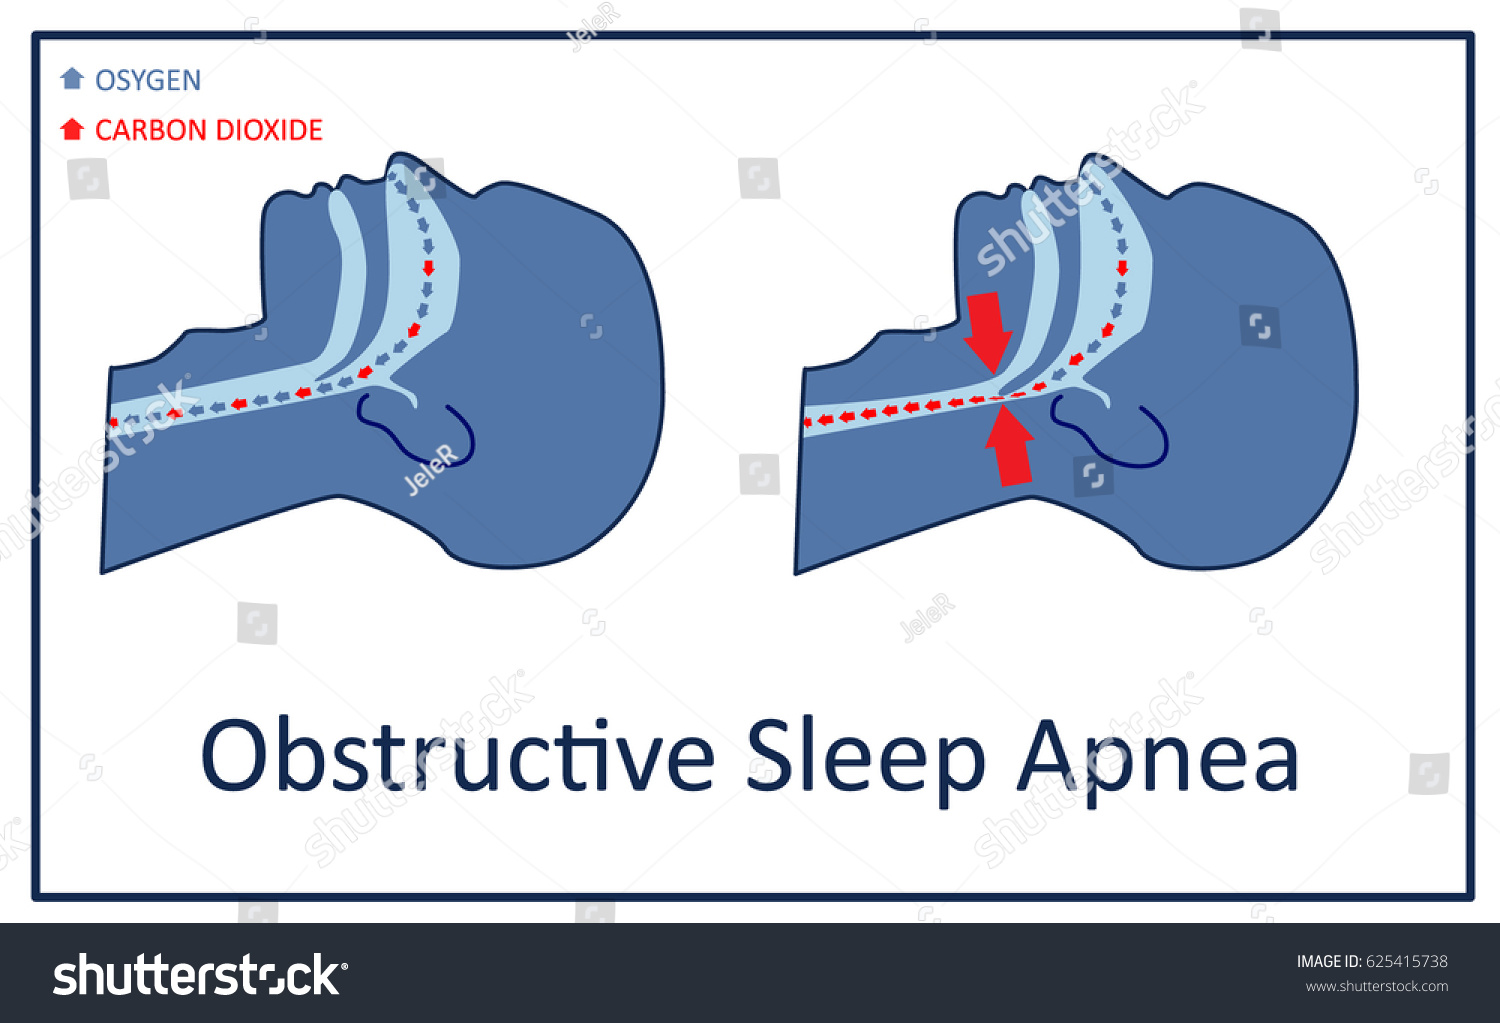
\includegraphics[height = 9cm]{stock-vector-vector-illustration-of-obstructive-sleep-apnea-625415738.jpg}
    \par (Courtesy of shutterstock)

\end{columns}
\end{frame}

\begin{frame}{互為因果}
    \begin{columns}
    \column{0.15\textwidth}
    \column{0.23\textwidth}
%    \tikz \draw[fill=green!5] (-5cm,-3cm) rectangle (0.5\textwidth, -1\textwidth) 
%    node[pos=0.5, align=left]{
    \tikz \draw (0, 0) node[fill=green!5, text width=5cm]{\huge{
    睡眠障礙\\
    睡眠呼吸中止\\

    }
    };

    \column{0.17\textwidth}
    \tikzarrow{red}{互為因果}
%    $\Longleftrightarrow$

    
    \column{0.45\textwidth}
%    \tikz \draw[fill=yellow!5] (0,0) rectangle (0.5\textwidth, -1\textwidth) node[pos=0.5, align=left]{
    \tikz \draw (0, 0) node[fill=yellow!25, text width=7cm]{
    \huge{
    $\makebox[\linewidth]{男性更年期}$\\
    \vspace{0.2cm}
    \hline
    \vspace{0.1cm}
        胸悶心悸、潮熱盜汗\\
        夜尿、攝護腺肥大\\
        焦慮、煩躁、憂鬱\\
        睪固酮分泌減少\\
        免疫力下降\\
        性功能障礙\\
        }
    };
    \end{columns}
\end{frame}

%%

\begin{frame}{互為因果}
    \begin{columns}
    \column{0.15\textwidth}
    \column{0.23\textwidth}
%    \tikz \draw[fill=green!5] (-5cm,-3cm) rectangle (0.5\textwidth, -1\textwidth) 
%    node[pos=0.5, align=left]{
    \tikz \draw (0, 0) node[fill=green!5, text width=5cm]{\huge{
    睡眠障礙\\
    睡眠呼吸中止\\

    }
    };

    \column{0.17\textwidth}
    \tikzarrow{red}{互為因果}
%    $\Longleftrightarrow$

    
    \column{0.45\textwidth}
%    \tikz \draw[fill=yellow!5] (0,0) rectangle (0.5\textwidth, -1\textwidth) node[pos=0.5, align=left]{
    \tikz \draw (0, 0) node[fill=blue!5, text width=7cm]{
    \huge{
    $\makebox[\linewidth]{交感神經亢奮}$\\
    \vspace{0.2cm}
    \hline
    \vspace{0.1cm}
造成->高血壓\\
造成->代謝症候群\\
造成->糖尿病\\
進而演變為...\\
心腦血管受損\\
心律不整\\
腦中風\\
耳鳴\\
}
    };
    \end{columns}
\end{frame}

%%
\section{Method}
\subsection{睡眠醫學}


\begin{frame}{睡眠呼吸中止症候群 OSA}
%    \PSG
% \studygoal% This is a flow chart defined in beamerthemelumc.sty. You can try to play with it if you are familiar with 'tikz' package.
\begin{columns}{~}

\column{0.50\textwidth}

\tikz \node[font=\sffamily\bfseries,scale=2.3,anchor=south] at (0,-0.1) {發生的機轉};

\begin{outline}

\1 咽喉部的肌肉鬆弛、軟組織肥厚\\
\1 睡眠姿勢、平躺角度\\
~\\
\tikz \node[font=\sffamily\bfseries,scale=1.0,anchor=south] at (0,0) {OSA 是一個循環};
\1 整晚經常處在淺睡,睡睡醒醒的分段睡眠(sleep fragmentation)\\
~\\
\1 高頻、間歇的鼾聲,伴隨著呼吸暫時停止($\geq$10 sec)\\
    \2 造成交感神經亢奮、壓力荷爾升高
    \2 AHI = 每小時發生「呼吸障礙」的次數
    
(* AHI: Apnea Hypopnea Index)
\end{outline}

\column{0.45\textwidth}

\begin{tikzpicture}
\newcommand{\LineWidth}{15mm}
\newcommand{\Radius}{4cm}
\node[font=\sffamily\bfseries,scale=2.8,anchor=south] at (0,-0.5) {OSA};
\node[font=\sffamily\bfseries,scale=1.8,anchor=south] at (0,-1.5) {(AHI)};
% 6\textsigma on the center
%\node[font=\sffamily,scale=6,anchor=north] at (0,0.5) {OSA};
% segments 5 -> 6: 72 degree -> 60 degree
\foreach \X [count=\Y] in {gray!50, yellow!50!orange, cyan!50, red, gray, green}
{\draw[line width=\LineWidth,\X] ({90-(\Y-1)*60}:\Radius)
arc({90-(\Y-1)*60}:{90-(\Y)*60}:\Radius);}
%`,width={1.5*\LineWidth}

% yellow!50!orange, gray!50, green, cyan!50, gray, red
\foreach \X [count=\Y] in {gray!50, yellow!50!orange, cyan!50, red, gray, green}
{\draw[-{rtriangle[bend,length={0.65*\LineWidth}]},
line width=\LineWidth,\X]
({90-(\Y-0.5)*60}:\Radius)
arc({90-(\Y-0.5)*60}:{90-(\Y)*60-10}:\Radius);}

\foreach \X [count=\Y] in {大腦睡-肌肉鬆, 打鼾, 呼吸阻塞, 血氧降低, 大腦醒-肌肉緊, 血氧正常}{
%{\ifnum \Y=3 % && \Y=4% upright (flip) this word
 % \( \), \AND, \OR, \NOT  \or \Y=4
    \ifthenelse{\Y=3 \or \Y=4}{% clause A
        \fill[decoration={text along path, text={|\Large\bfseries| \X},
     raise=-3pt,text color=black,text align=center},decorate]
     ({90-(\Y)*60-5}:\Radius)
    arc({90-(\Y)*60-5}:{90-(\Y-1)*60-5}:\Radius);
    }{% clause B
        \fill[decoration={text along path, text={|\Large\bfseries| \X},
     raise=-3pt,text color=black,text align=center},decorate]
     ({90-(\Y-1)*60-5}:\Radius)
    arc({90-(\Y-1)*60-5}:{90-(\Y)*60-5}:\Radius);
    }
%\fi }
} % end foreach

\end{tikzpicture}

\end{columns}

\end{frame}


\begin{frame}{診斷睡眠呼吸中止}
\begin{columns}
    \column{0.45\textwidth}
%    \begin{block}
        \begin{outline}
        \1 Polysomnography (PSG) 在醫院「睡眠多項生理檢查」,蒐集:
        \2 腦波圖、口鼻呼吸氣流、血氧濃度(SpO2)、鼾聲、肌電圖
        \2 計算 AHI

        \end{outline}
%    \end{block}
~\\    
~\\
~\\
~\\
~\\
~\\
%    \begin{block}
        \begin{outline}
%    \1 睡眠呼吸中止症候群 (OSA)
        \1 看「面相」,量體重(BMI $> 30$)
        \1 鼻腔跟口咽檢查(Mallampati score 3 or 4),醫學影像
        \2 cephalometry, cone-beam CT scan, MRI
        \1 內視鏡觀察睡眠中口咽狀態 (Drug Induced Sleep Endoscopy, DISE) 
    \end{outline}
%    \end{block}
%    \begin{block}
    
%    \end{block}
    \column{0.15\textwidth}
    \textcolor{red}{AHI} 指數(apnea-hypopnea index) $=$ 睡眠呼吸障礙事件的次數/小時
    ~\\
    ~\\
        \centering

        \begin{tikzpicture}% based on https://tex.stackexchange.com/a/9561/ (Caramdir's fantastic answer to another question)
        \node (tiger) [anchor=south west, inner sep=0pt] {        
\includegraphics[width=0.7\textwidth]{stock-vector-full-length-male-silhouette-body-human-figure-thin-fat-and-athletic-man-vector-illustration-obesity.jpg}};
        \begin{scope}[x={(tiger.south east)},y={(tiger.north west)}]
          \foreach \i/\j in {{(0.35,0.75)/(-0.35,0.2)}, %RF
        {(0.65,0.85)/(1.15,1.00)}, %LH
        {(0.66,0.7)/(1.15,0.2)}, %LF
        {(0.35,0.85)/(-0.35,1.01)}} % RH
            \draw [red, thick] \i -- \j;
        \end{scope}
      \end{tikzpicture}

    \column{0.40\textwidth}
%    \begin{block}
        \begin{outline}
        \1 居家睡眠檢查 (home sleep testing, HST)
        \2 AHI 來自口鼻呼吸氣流、血氧濃度(SpO2)、鼾聲、胸腹呼吸動作
        \end{outline}
%    \end{block}
~\\
~\\
~\\
~\\
~\\

%    \begin{block}
        \begin{outline}
        \1 HRV 心律變異($\less 50$ 代表交感神經活性太高)
        \1 睡眠品質量表、夜尿量表
        \2 The Functional Outcomes of Sleep Questionnaire (FOSQ)
        \2 The Epworth Sleepiness Scale (ESS)
        \end{outline}
%    \end{block}

\end{columns}

%\setlength{\unitlength}{1cm}
%\thicklines
%\draw (3,8) -- (5,6)
%\put(3,8){\line(3,-2){3}} % start at (3,8) toward (3,-2) with length 3 cm
    
\begin{block}{關鍵字:}
\footnotesize{
Obstructive Sleep Apnea (OSA) 睡眠呼吸中止, Sleep Surgery, Palatopharyngoplasty, Algorithm, Maxillomandibular Advancement, Hypoglossal Nerve Stimulation, Upper Airway Stimulation}  
    \end{block}


\end{frame}


\begin{frame}{治療睡眠呼吸中止症候群}

\begin{adjustbox}{minipage=15cm, center}


% Requires the booktabs if the memoir class is not being used
\resizebox{1\linewidth}{!}{
\begin{table}[htbp]
   \centering
   %\topcaption{Table captions are better up top} % requires the topcapt package
   \begin{tabular}{@{} llll @{}} % Column formatting, @{} suppresses leading/trailing space
      \toprule
      \multicolumn{4}{c}{AHI} \\
      \cmidrule(r){2-4} % Partial rule. (r) trims the line a little bit on the right; (l) & (lr) also possible
      &	輕度&	中度	&	重度\\
      建議    & \textcolor{red}{5}-14.9 & \textcolor{red}{15}-29.9	& \textcolor{red}{30}-\\
      \midrule
      首選	&	減重	&	減重	&	減重\\
                      &  睡姿*    &   &\\
       保守     &  & 陽壓呼吸器  &	陽壓呼吸器\\

             & 止鼾牙套  & 止鼾牙套 & 止鼾牙套\\
                             &      &   &\\
      手術       &   & 鼻中膈與咽 &		鼻中膈與咽\\
       &   & 	正顎手術  &	正顎手術\\
      \bottomrule
      \multicolumn{4}{c}{\small *睡眠姿勢,上半身壂高30度(氣流易通過)}\\
   \end{tabular}
%   \caption{Remember, \emph{never} use vertical lines in tables.}
   \label{tab:booktabs}
\end{table}
} % end of \resizebox
\end{adjustbox}
\end{frame}



\begin{frame}{治療睡眠呼吸中止症候群}
%\begin{adjustbox}{minipage=5cm, center}
%\begin{block}
\begin{columns}[onlytextwidth]

%\column{0.02\textwidth}

\column{0.70\textwidth}{\huge{依照流程與次第}}
%\begin{figure}
%    \centering
    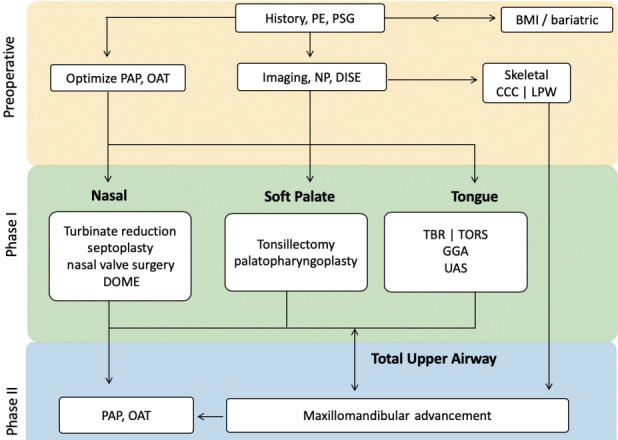
\includegraphics[height = 12cm]{ceo-2020-01053f6.jpg}
    \par (Courtesy of Liu et. al., 2020. Surgical algorithm for obstructive sleep apnea: An update. Clinical and Experimental Otorhinolaryngology vol. 13 215–224)
%\end{block}

\column{0.25\textwidth}
    \par Updated Stanford sleep surgery algorithm. PE, physical examination; PSG, polysomnography; BMI, body mass index; PAP, positive airway pressure; OAT, oral appliance therapy; NP, nasopharyngoscopy; DISE, drug-induced sedation (sleep) endoscopy; CCC, complete con- centric collapse; LPW, lateral pharyngeal wall; DOME, distraction osteogenesis maxillary expansion; TBR, tongue base reduction; TORS, tran- soral robotic surgery; GGA, genioglossus advancement; UAS, upper airway stimulation.\\
%    \label{fig:my_label}
%\end{figure}
\end{columns}

%\end{adjustbox}

\end{frame}

\begin{frame}{第一方案}
減重\\
配合 oral myofunctional therapy\\
台北慈濟醫院語言治療師蔡得榕\\
舌底肌群愈強壯, 睡眠時依舊能維持紮實的外形(muscular consistency)\\
tongue training by protruding: 舌前伸 10 sec\\
%\url: https://www.youtube.com/watch?v=f5FXSpkT9pk
%x https://www.youtube.com/channel/UCQRtGEdMoQXdH-WHMGufKig

%音樂治療師
\end{frame}

\begin{frame}{第二方案 CPAP}
    \centering
    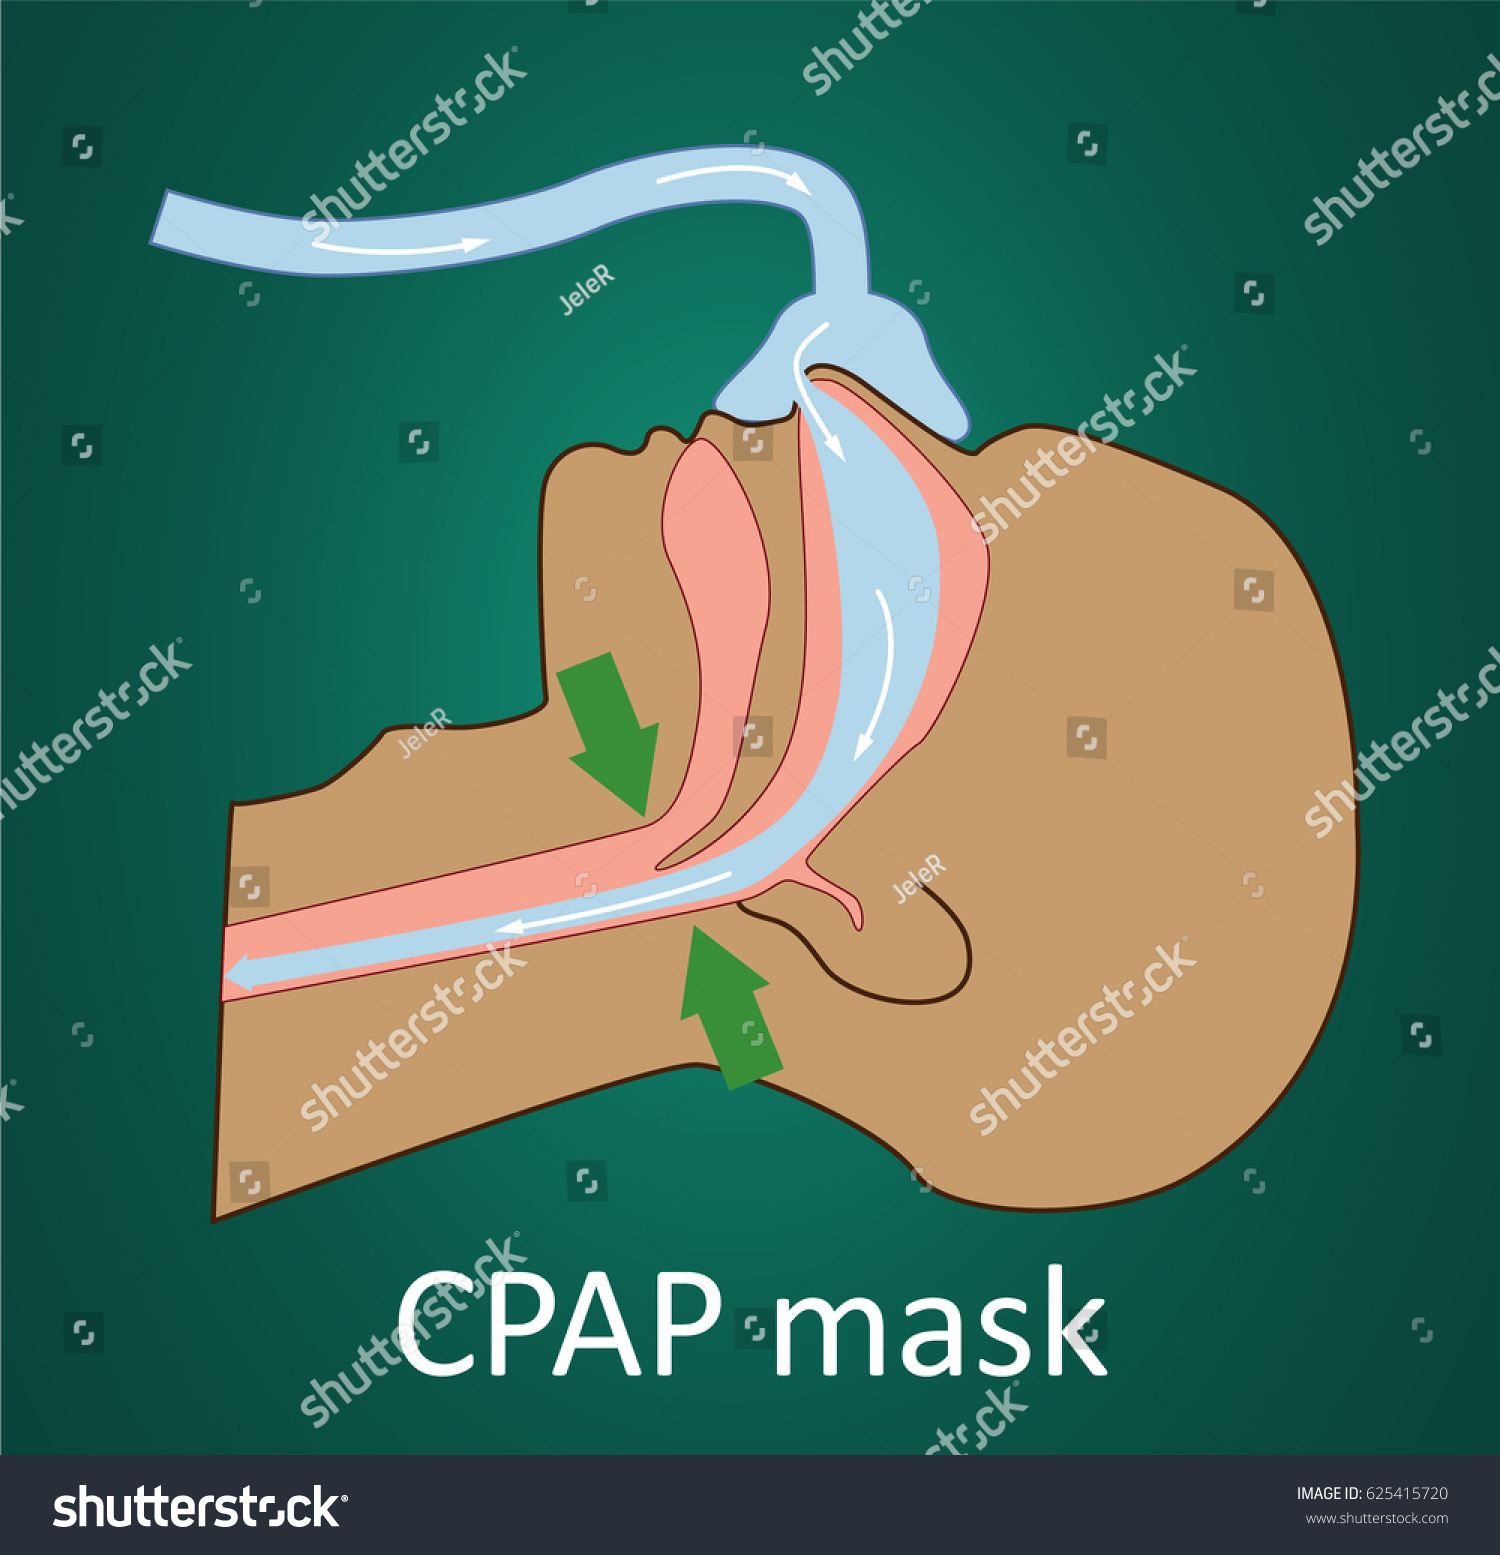
\includegraphics[height=0.30\textwidth]{stock-vector-vector-illustration-of-normal-breathing-with-cpap-mask-625415720.jpg}
    
    \begin{block}{CPAP: continuous positive airway pressure}
    「陽壓呼吸器」,入睡時配戴於口鼻(或僅鼻),提供咽喉正向壓力,防止塌陷。由睡眠技師調整參數,尋求最適當的壓力、溫度、濕度,減少刺激與鼻塞。也有吐氣時降壓等自動調節功能,減少配戴時的不適。亦能同步監測(手指)血氧濃度(SpO2)。
    \end{block}

\end{frame}

\begin{frame}{第三方案: OAT 止鼾牙套}
\centering
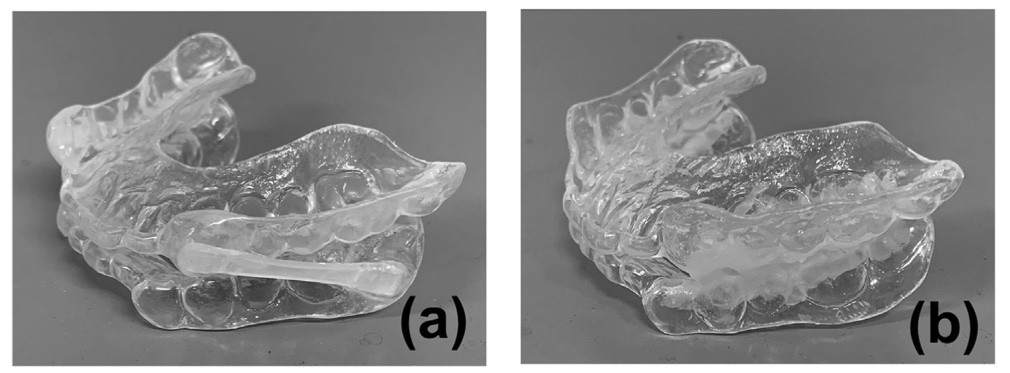
\includegraphics[height=0.30\textwidth]{Yanamoto2021.jpg}
\par Courtesy of Yanamoto, S. et al.(2021) Semi-fixed versus fixed oral appliance therapy for obstructive sleep apnea: A randomized crossover pilot study. J. Dent. Sci. 16, 404–409: The oral appliance. (a) The semi-fixed oral appliance was comprised of two lateral connectors and individual customized appliances for the maxilla and mandible. (b) The fixed oral appliance consisted of appliances fixed together with resin.


\begin{block}
Oral appliance therapy (OAT)\\
by
Mandibular advancement devices (MADs)\\
anti-snoring guard 止鼾牙套 周孫隆老師\\

Adjustable devices
* Thornton anterior positioner (TAP)

* Dynamax mandibular device

    主要有4種designs, 
attached: bilateral traction , bilateral compression, anterior traction 
unattached : bilateral interlocking. 
看病人的dentition 狀況決定何種設計: 如severe bruxism , muscle capsule 很緊以anterior traction 為主( 但嚴重的anterior attrition 就不適合) 
Muscle tone 很弱, 睡著時mandible 很容易會往後塌陷, 以bilateral traction 為主⋯⋯⋯⋯( 很多考量, 所以有機會可以和主任討論) 

決定好主要設計後再來看retention 要放哪裡(就是propulsion 設計, 以tooth number, tooth Andre, tooth shape 來考量) 

最後就是看一開始前置的量, 首先先決定maximal range of movement ( 即確認病人能夠最前置的量再加上overjet (如測量U1-L1 水平距離最大可達8mm, 病人overjet 是4mm. 那麼他的ROM 是12mm) 
AADSM 建議若沒有其他考量, 則一開始可以放在50\%-75\% ROM 的量。再以每個月0.5-1 mm 做titration
\end{block}

\end{frame}

\begin{frame}{有可能必要的方案}
    \begin{columns}
    
    \column{0.7\textwidth}
    \begin{outline}
    \1<1-> 手術處理: 擴大呼吸道
        \2<2-> 軟組織
            \3<3-> 鼻腔
            \3<4-> 咽喉
            \3<5-> 舌根(除去黑圈部位)
        \2<6-> 硬組織(上、下顎骨)
    \end{outline}
    
    \column{0.3\textwidth}    
    \centering
    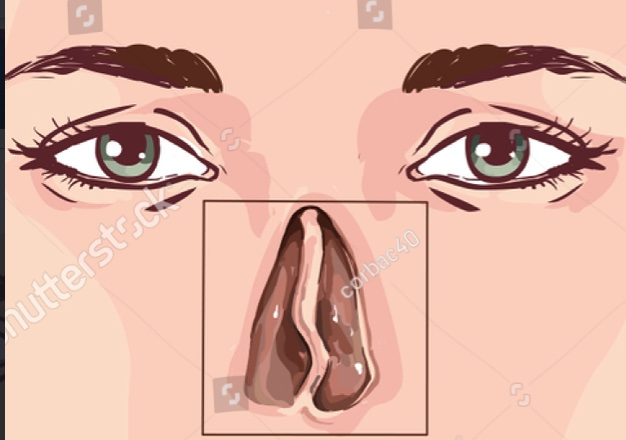
\includegraphics[width=0.9\textwidth]{nasal_septum.jpg}\only<3>
    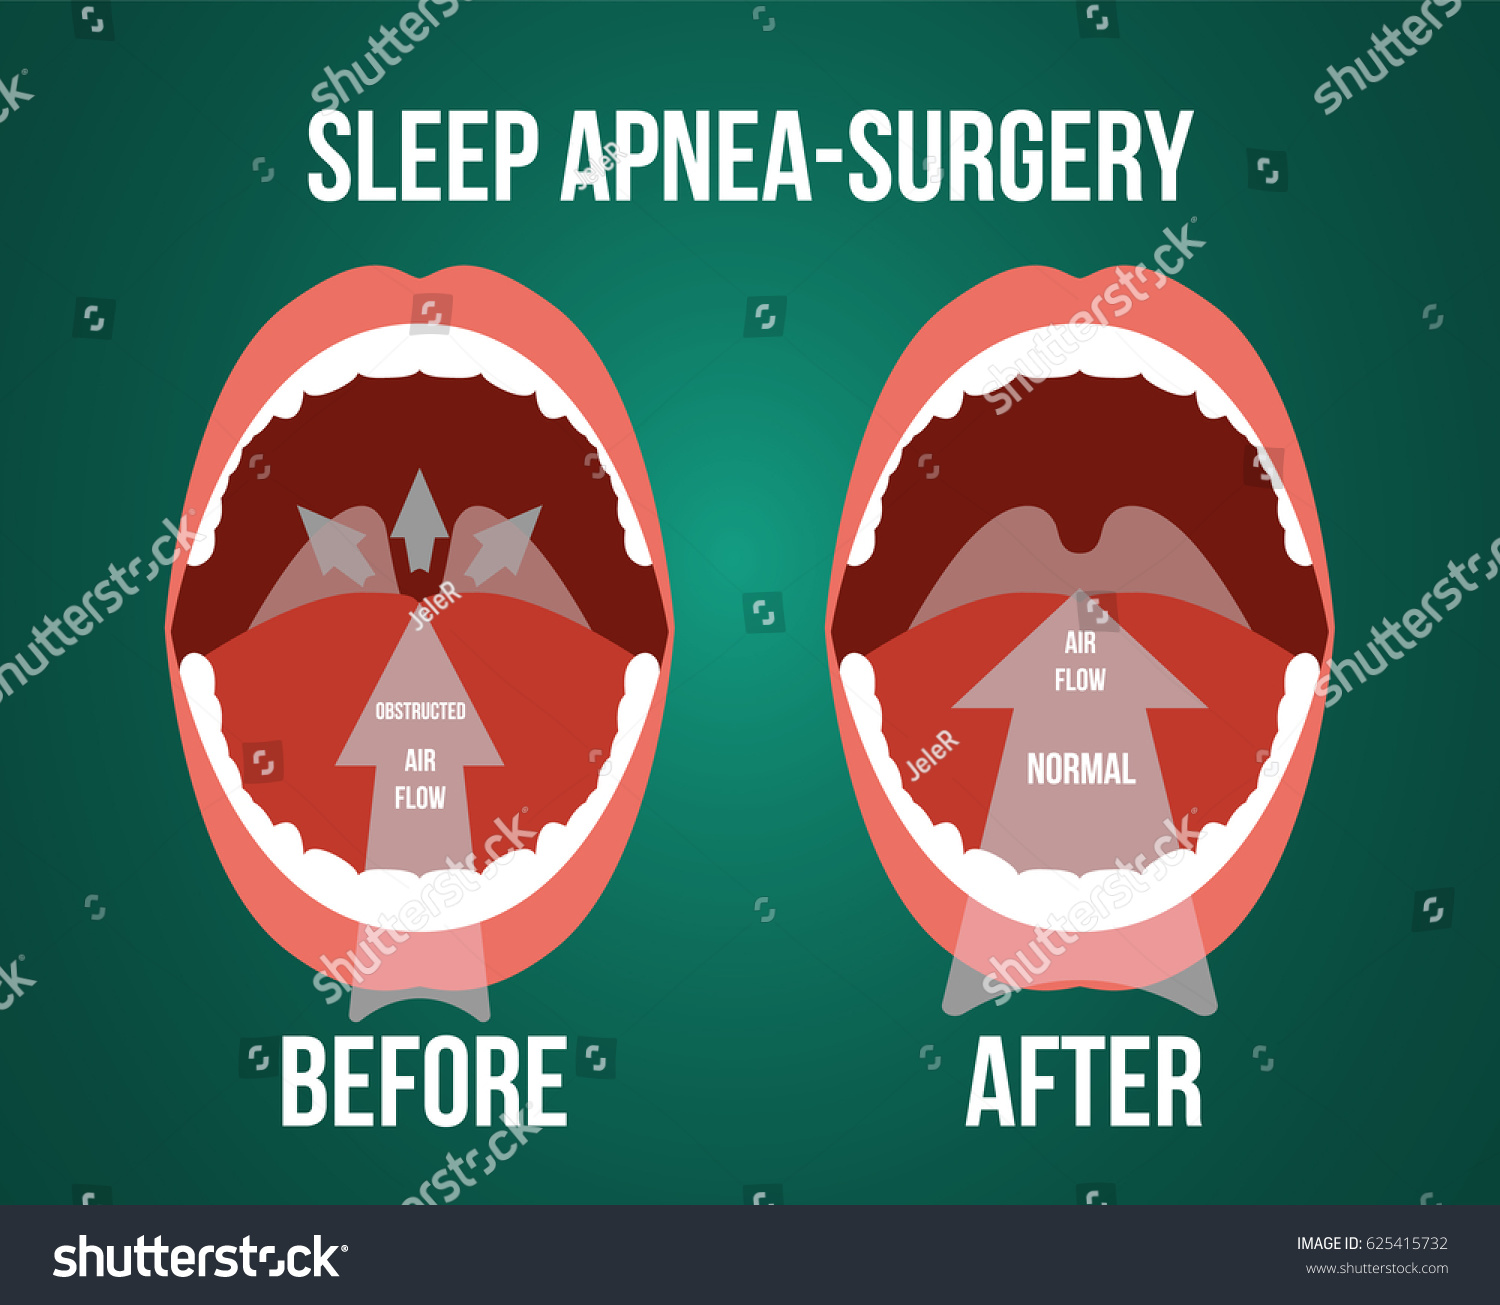
\includegraphics[width=0.9\textwidth]{stock-vector-vector-illustration-of-surgery-for-obstructive-sleep-apnea-before-and-after-result-625415732.jpg}\only<4>
    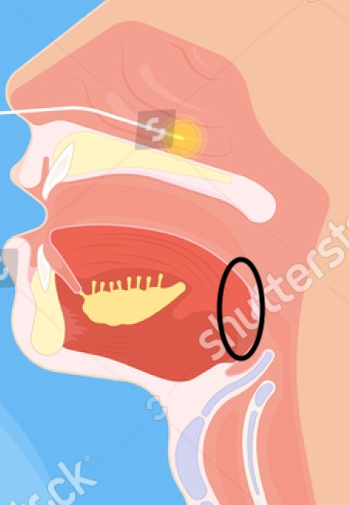
\includegraphics[width=0.9\textwidth]{tongue_base.jpg}\only<5>
    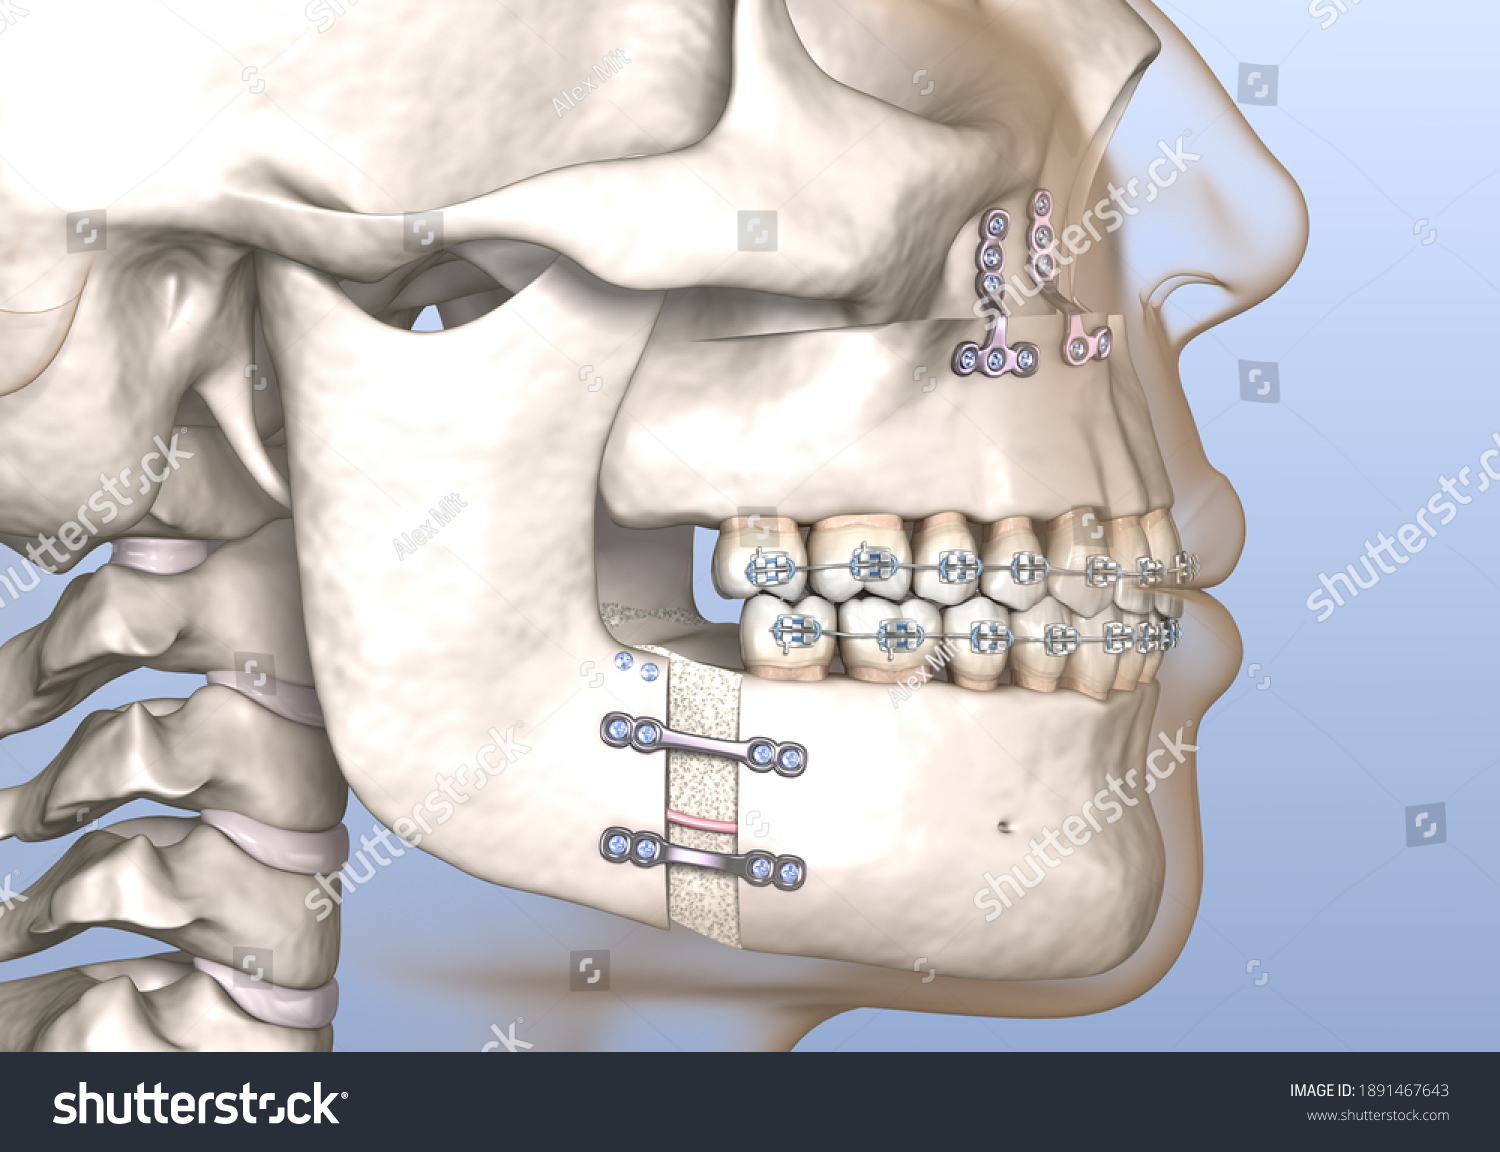
\includegraphics[width=0.9\textwidth]{stock-photo-maxillomandibular-advancement-surgery-medically-accurate-dental-d-illustration-1891467643.jpg}\only<6>
%    \includegraphics[]{}<1->
    \end{columns}
\end{frame}

\begin{frame}{Method for A good Sleeping}
\begin{block}{全人睡眠醫學團隊}
%\centering
%$\log a \cong  \beta_2\text{\bf ln~}
%b + \beta_1 x_t + \beta_0$\par\\
睡眠中心PSG 睡眠檢查(神經內科 黃志善、宋家瑩醫師)
居家睡眠檢查(Home Sleep Test)(科林)
耳鼻喉科及睡眠醫學專科醫師:林伯岳醫師(鼻與喉軟組織手術)
口腔顎面外科:祁力行醫師(正顎手術,雷射針灸)、侯俊羽醫師(正顎手術)
—周珊如 anti-snoring guard
(牙科部李勝揚主任的齒列矯正互相搭配)
distraction osteogenesis maxillary expansion [DOME]
~~\\
%\centering
%\includegraphics<2>[width = %10cm]{im/chd1}
\end{block}
\end{frame}


\begin{frame}{Data and results}
\subsection{全人睡眠照護}
\begin{block}{訣竅}
~~\\
要做\\
~~\\
運動減重(脖圍$< 43 cm$)\\
傍晚運動有利於增加睪固酮,減少壓力荷爾蒙可體松,並改善脂肪囤積(肥胖)\\
維持舒適的睡眠環境(光音熱、氣味、氣氛及心情)\\
睡眠是重要的儀式(安靜下來,告訴身體準備就寢,每天要定時)\\
每天22:00-06:00是最佳睡眠時段\\


~~\\

不要做\\
~~\\
白天小睡少於30分鐘\\
避免睡前菸、酒、咖啡、茶、藍光(手機)\\
少量飲水\\
避免睡前進食、劇烈運動(四小時內)\\
~~\\
~~\\
\end{block}
\end{frame}

\begin{frame}
~~\\
~~\\
中醫
1)中醫臨證,對症下藥輔佐減重、針灸減重(如果患者害怕毫針,我也可以做 RJ laserpen 低能量雷射針灸減重)。
(雷射)針灸也能幫助提升睡眠品質。
中醫十問正是全人照護的標準模型。

2) 中醫針灸戒菸門診 ( 理由是 OSA in current smokers may be more severe 吸菸會讓睡眠呼吸中止,更加嚴重),而且戒菸者體重容易增加,需要飲食、運動、中藥、針灸幫忙控制體重。

3) 中藥熏鼻
黃中瑀主任,想推行中藥熏鼻很久了(自費水藥,賣點在於不是類固醇、不是 anti-histamine ,芳香氣味可以選擇),(他們稱為:御醫配方,因為皇帝們的中藥挑選氣味、口味,配不好御醫別幹了) (Happy)
需要使用加熱機器,揮發藥水

4) 雷射針灸、肌肉筋膜與顳顎關節障礙
雷射針灸能幫助提升睡眠品質。

~~\\
~~\\
\end{frame}

\subsection{全人中醫}% you can start a subsection in a slice

\begin{frame}
    \begin{outline}
\1 RJ Laserpen 雷射針灸

\2 穴位:內關 (安神止胸悶)
\2 穴位:下關 上關 頰車 
\2 穴位:風池 揉法 
\2 穴位:合谷 曲池 三陰交 下巨虛 上巨虛 足三里 陽陵泉 豐隆 犢鼻 

\1 Further follow up (HRV; liver massage for body-mind connection) at TMWH (W3 pm 睡眠整合門診 for home sleep 
\2 monitor and weight reduction)
\2 quit e-cigarette at future by 中藥水開鼻竅 (3mL per day)
    \end{outline}

%\begin{block}{Results}
%\centering
%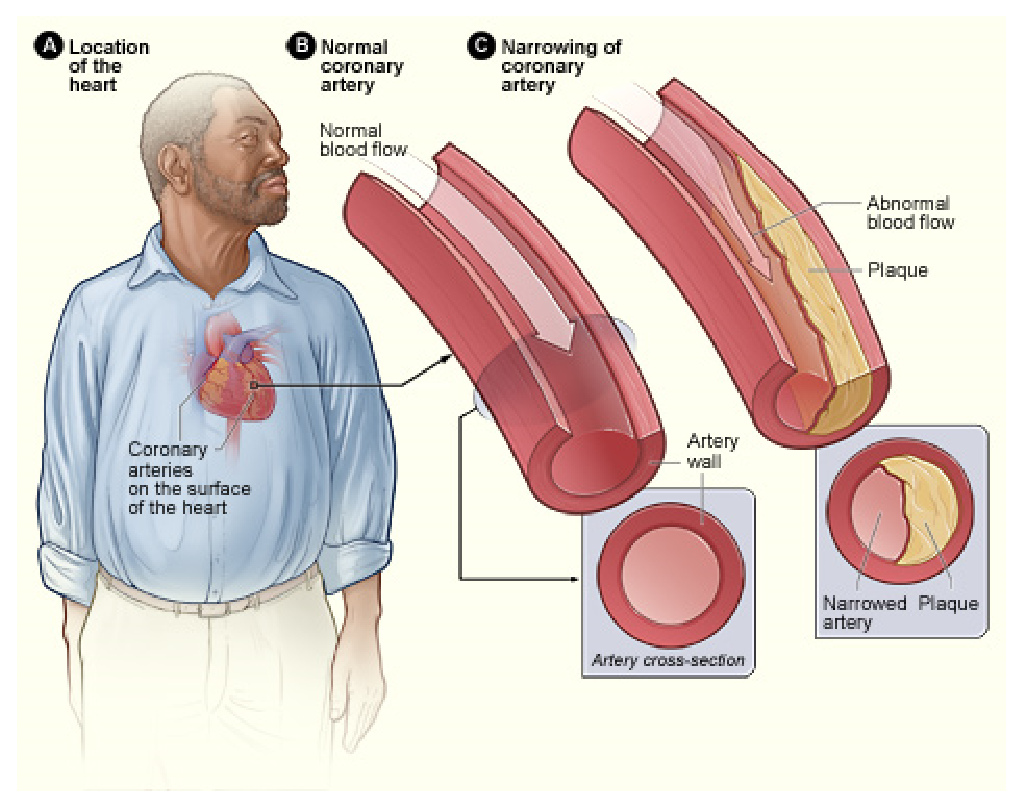
\includegraphics[height =10cm]{im/chd1}
%\end{block}

\end{frame}

\begin{frame}
66歲 鄧傳鈺先生,若來看診,請多關照,感謝!
Wednesday, June 16
\end{frame}





\section{Discussion}
\begin{frame}{~}
\begin{columns}[onlytextwidth]
\column{0.02\textwidth}
\column{.9\textwidth}
\begin{block}{Discussion}
~~\\
~~\\
\begin{itemize}
\item point 1
\vskip0.5cm
\item point 2
\vskip0.5cm
\item point 3 
\vskip0.5cm
\item point 4
\vskip0.5cm
\item point 5
\vskip0.5cm
\item point ...
\vskip0.5cm
~
\end{itemize} 
\end{block}
\column{0.02\textwidth}
\end{columns}
\end{frame}
%\section{Update of the work}


\section{Acknowledgments}
\begin{frame}{Acknowledgments}

\begin{columns}[onlytextwidth]
\column{0.02\textwidth}
\column{.45\textwidth}

\begin{block}{耳鼻喉科}
\begin{itemize}
\vskip0.5cm
\item 林伯岳醫師 
\vskip0.5cm
\item name 
\end{itemize}
\vskip1.7cm
~
\end{block}
\vskip1cm 

\begin{block}{口腔顎面外科}
\vskip0.5cm 
\begin{itemize}
\item name
\vskip0.5cm
\item name 
\end{itemize}
\vskip1.7cm
~
\end{block}

\column{.45\textwidth}
\begin{block}{睡眠醫學中心}
\vskip0.5cm 
\begin{itemize}
\item 神經內科 
\vskip0.5cm
\item 胸腔內科 
\vskip0.5cm
\item 精神科
\vskip0.5cm
\item 心臟內科
\vskip0.5cm
\item 臨床心理師
\vskip0.5cm
\item 睡眠技術員
\vskip0.5cm
減重中心
\vskip0.5cm
戒菸門診
\end{itemize}

\end{block}
\vskip1cm
\begin{block}{神經內科、胸腔科、耳鼻喉科、精神科、心臟科及口腔顎面外科,臨床心理師、睡眠技術員}
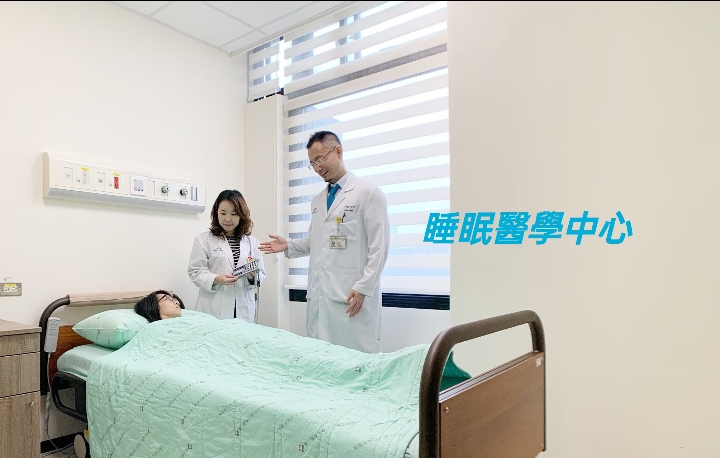
\includegraphics[height=0.4\textheight]{CostUnitImage1202104151044255.jpg}%
\end{block}
\column{0.02\textwidth}
\end{columns}


\end{frame}

\begin{frame}[label={lastframe}]
\end{frame}

%\end{CJK*}

\end{document}